\documentclass[12pt]{article}

\usepackage[T1]{fontenc}
\usepackage{lmodern}
\usepackage{titling}
\usepackage{graphicx}
\graphicspath{{./images/}}
\usepackage{subcaption}
\usepackage[none]{hyphenat}
\usepackage{mathtools}
\usepackage{hyperref}
\usepackage{float}
\usepackage{microtype}
\usepackage{tikz}
\newcommand*\circled[1]{\tikz[baseline=(char.base)]{
		\node[shape=circle,draw,inner sep=0pt] (char) {#1};}}

\usepackage
[
a4paper,% other options: a3paper, a5paper, etc
left=2cm,
right=2cm,
top=4cm,
bottom=4cm,
% use vmargin=2cm to make vertical margins equal to 2cm.
% us  hmargin=3cm to make horizontal margins equal to 3cm.
% use margin=3cm to make all margins  equal to 3cm.
]
{geometry}
\setlength{\droptitle}{-10em}

\title{Coursework 1}
\author{Dobrik Georgiev \\ \small dgg30@cam.ac.uk}

\begin{document}

\maketitle
~\\
\textit{\circled{1.} Describe each one of the potential limitations of multiplexing
and the advantages of carrier sensing medium access.}

Multiplexing is a way to share the medium by splitting into different time
frames (time multiplexing) or frequency bands (frequency multiplexing) or some
other way. However, depending on traffic some users may want to send more or
less data, which cannot be handled just by multiplexing.

CSMA on the other hand first senses the medium and if sensed idle transmits the
data. With Collision Avoidance (CA) (or CSMA/CD for ethernet) and even MACA to
solve the hidden terminal problem it would avoid data collisions quite
effectively. Also exponential back-off schemes lower probabilites of collisions
re-occurring but also allows for full use of the channel, when sensed idle.
\\
\\
\textit{\circled{2.} Collision detection schemes employed in fixed network MAC protocols do not work in wireless
networks. Explain (using diagrams) hidden terminal and exposed terminal problems and present
possible solutions. Particularly, how is collision detection implemented in 802.11?}

Consider the following scenario:
\begin{figure}[H]
    \centering
    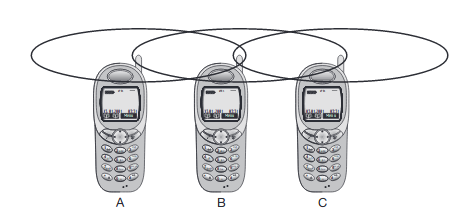
\includegraphics[width=250pt]{hidden_terminal.png}
\end{figure}
The transmission range of A reaches B, but not C (the detection range does
notreach C either). The transmission range of C reaches B, but not A. Finally,
thetransmission range of B reaches A and C, i.e., A cannot detect C and vice
versa

A starts sending to B, C does not receive this transmission. C also wants
to send something to B and senses the medium. The medium appears to be free, the
carrier sense fails. C also starts sending causing a collision at B. But
A cannot detect this collision at B and continues with its transmission. A is
\textbf{hidden} for C and vice versa.

While hidden terminals may cause collisions, the next effect only
causes unnecessary delay. Now consider the situation that B sends something to
A and C wants to transmit data to some other mobile phone outside the
interference ranges of A and B. C senses the carrier and detects that the
carrier is busy (B's signal). C postpones its transmission until it detects the
medium as being idle again. But as A is outside the interference range of C,
waiting is not necessary. Causing a `collision' at B does not matter because the
collision is too weak to propagate to A. In this situation, C is
\textbf{exposed} to B.

Multiple access with collision avoidance (\textbf{MACA}) presents a solution to
the hidden terminal problem. Consider the same scenario as before:
\begin{figure}[H]
    \centering
    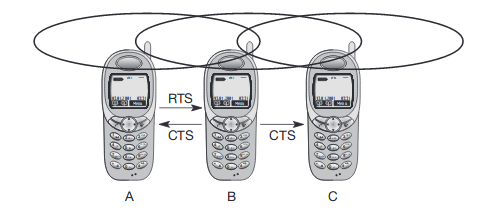
\includegraphics[width=250pt]{hidden_terminal_soln.png}
\end{figure}
With MACA, A does not start its transmission at once, but sends
a \textbf{request to send (RTS) first}. B receives the RTS that contains the
name of sender and receiver, as well as the length of the future transmission.
This RTS is not heard by C, but triggers an acknowledgement from B, called
\textbf{clear to send (CTS)}. The CTS again contains the names of sender (A)
and receiver (B) of the user data,and the length of the future transmission.
This CTS is now heard by C and the medium for future use by A is now reserved
for the duration of the transmission. After receiving a CTS, C is not allowed
to send anything for the duration indicated in the CTS toward B. A collision
cannot occur at B during data transmission, and the hidden terminal
problem is solved, provided that the transmission conditions remain the
same. Still, collisions can occur during the sending of an RTS, but since 
RTS is very small compared to data transmission, the probability of collision
is much lower. No transmission is allowed without the appropriate CTS.

Can MACA help to solve the exposed terminal:
\begin{figure}[H]
    \centering
    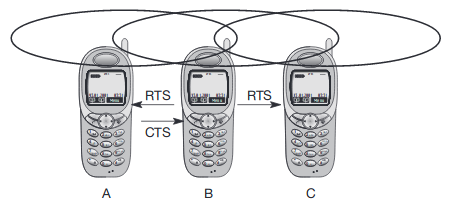
\includegraphics[width=250pt]{exposed_terminal.png}
\end{figure}
B has to transmit an RTS first containing the name of the receiver (A) and the
sender (B). C does not react to this message as it is not the receiver, but
A acknowledges using a CTS which identifies B as the sender and A as the
receiver of the following data transmission. C does not receive this CTS and
concludes that A is outside the detection range. C can start its transmission
assuming it will not cause a collision at A.

(For this I assume you meant collision \emph{avoidance}.) As for 802.11 I think
it uses the same logic for RTS and CTS, but: (i) a node waits for a specified
length of time (SIFS/PIFS/DIFS, SIFS<PIFS<DIFS); (ii) if sensing medium is
busy, waits again same time + random exponential backo-off.
\\
\\
\textit{\circled{3.} Describe the essential differences between standard ad-hoc
routing protocols and delay tolerant routing.}

In ad-hoc networks you have `end-to-end' connectivity assured, i.e. no storage
on intermediate nodes is needed. However, the topology of the network will be
constantly changing as nodes move around.

In a \textbf{Delay Tolerant Network (DTN)} you have the same conditions as
above, but the connectivity is even more limited, there are isolated nodes and
communication is often short and sporadic. With DTN you cannot assume
end-to-end connectivity, so nodes need to store the data for as long as
necessary and forward it, when provided with an opportunity (as in the example
with epidemic routing).
\\
\\
\textit{\circled{4.} Discuss in detail differences between infrastructure mode
and ad hoc mode in wireless networks.}

Most Wi-Fi networks function in infrastructure mode. All devices on the network
communicate through a single \textbf{Access Point (AP)}, which is usually the
wireless router. Even if the two devices are right next to each other, they
will communicate through the AP. Infrastructure mode is ideal if you are
setting up a more permanent network and would require you to purchase an AP.

In ad-hoc mode, each device communicates directly with each other. There is no
centrall AP which controlls device communication, i.e. it is peer-to-peer.
Ad-hoc mode can be easier to set up if you just want to connect a handful of
devices to each other (or if you are in a cheap hotel without Wi-Fi but want to
connect two laptops to each other). However, ad-hoc mode would require that
devices pass the data through each other (no AP, remember) if they are not
directly connected, which is slower than the Infrastructure mode option.

(I can't seem to find any further details...)
\\
\\
\textit{\circled{5.} Routing in mobile networks can be adapted from fixed
network routing. Describe a proactive and a reactive routing scheme for an
ad-hoc network. What are the problems in using such protocols in a DTN?}

Proactive: \textbf{Destination sequence distance vector (DSDV)}\\
Each node maintains a table with a route to every node and each entry of the
table has a sequence number assigned by the destination:
\begin{figure}[H]
    \centering
    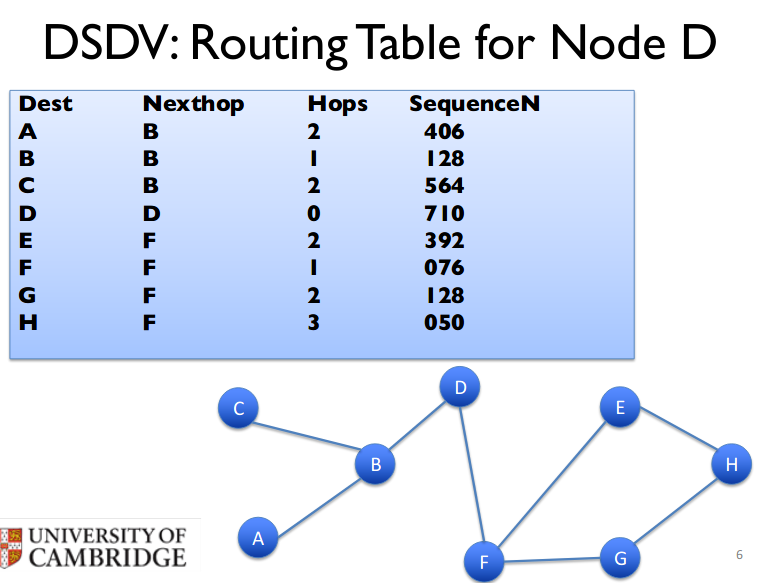
\includegraphics[width=250pt]{dsdv_table.png}
\end{figure}
Each node exchanges its neighbor table periodically (to be more precise,
exchanges the updates) with its neighbors and changes at one node propagate
through the network. The node includes its sequence number with the update.
When two routes to a destination from two different neighbours are received,
the one with greatest destination sequence is chosen, in order to prevent
loops.

Reactive: \textbf{Dynamic Source Routing (DSR)}\\
Dynamic source routing (DSR), divides the task of routing into two
separate problems:
\begin{itemize}
    \item \textbf{Route discovery:} A node only tries to discover a route to
        a destination if it has to send something to this destination and there
        is currently no known route.
    \item \textbf{Route maintenance:} If a node is continuously sending packets
        via a route, it has to make sure that the route is held upright. As
        soon as a node detects problems with the current route, it has to find
        an alternative.
\end{itemize}
If a node needs to discover a route, it broadcasts a route request with
a unique identifier and the destination address as parameters. Any node that
receives a route request does the following:
\begin{itemize}
    \item If the node has already received the request (which is identified
        using the unique identifier), it drops the request packet.
    \item If the node recognises its own address as the destination, the request
        has reached its target.
    \item Otherwise, the node appends its own address to a list of traversed
        hops in the packet and broadcasts this updated route request.
\end{itemize}
As soon as the request reaches the destination, it can return the request packet
containing the list to the receiver using this list in reverse order. One
condition for this is that the links work bidirectionally. If this is not the
case, and the destination node does not currently maintain a route back to the
initiator of the request, it has to start a route discovery by itself. Sequence
numbering could be used as in DSDV to prevent looping.

The problem with these two protocols is that they do not assume storage on
intermediate nodes. Therefore, if there is no connected path between two nodes
for long enough transmission between the two nodes would be impossible.
\\
\\
\textit{\circled{6.} Compare and contrast Epidemic routing and Probabilistic
routing, with respect to overhead, latency and delivery success ratio. When is
Epidemic routing not beatable as a delay tolerant protocol?}
(I'm not sure Probabilistic routing has been taught.)
\\
\\
\textit{\circled{7.} Compare preamble sampling protocols (XMAC) to SMAC.}

Both are duty cycling protocols, designed for wireless sensor networks where
energy consumption is the primary goal. Measurements have shown that idle
listening consumes as much power as transmission. Both protocol try to reduce
energy waste. SMAC is synchronous, XMAC not, as it will become obvious below.

Given these facts, it is not necssary to keep nodes listening all the time, and
thus SMAC reduces the listen time by putting nodes into \emph{periodic} sleep
state. In the sleep state the radio is completely turned off. Each node for
some sleeps for some time and then wakes up and listens to see if any other
node wants to talk to it. During sleeping the node turns off its radio and sets
a timer to wake up. All nodes are free to choose their own listen/sleep
schedules, but to reduce control overhead, we prefer neighbouring nodes to
synchronise together -- they listen at the same time and go to sleep at the
same time. (Not all neighbouring nodes can synchronise together!) Nodes
exchange their schedules periodically by broadcasting a SYNC packet to their
intermediate neighbours. A node talks to its neighbours at their schedulet
listen time.

For collision avoidance (apart from the RTS/CTS scheme), there is a duration
field in each transmitted packet that indicates how long the remaining
transmission will be.  Upon receiving a packet to another node, the receiver
will node how long to keep silent from this field. Tthe node records this value
in the \textbf{Network Allocation Vector (NAV)} and sets a timer for it. On
each timer tick the NAV is decremented, until it reaches 0. Before initiating
a transmission a node first looks at the NAV, if it is >0, the node determines
the medium is busy.

XMAC (and LPL), on the other hand, do not try to explicitly synchronise nodes,
but use preambles instead. With this technique nodes periodically wake up to
sample the wireless channel for any activity. If energy is detected on the
channel, the node remains awake in order to receive a packet. Otherwise, the
node quickly goes back to sleep. To minimize overhead when the network is idle,
these periodic wakeups are not synchronized across nodes: that is, the sender
knows the recipient's wakeup interval but not its wakeup time. Accordingly,
before transmitting a packet, the transmitter sends a preamble stream at least
as long as the recipient's wakeup interval (in the case of LPL); this ensures
that the recipient will sample the channel during the preamble. After the
preamble, the sender and recipient exchange data packets. In the case of XMAC,
the `preamble communication' is instead modified by inserting destination
address information and it is split in periodic streams of short preambles.
When a node wakes up, it may decode the destination address and see if it is
the intended recipient. If so, it uses the gaps in the preamble to send an ACK
to the sender, which will in turn immediately transmit the payload.

In terms of performance, SMAC trades off energy consumtion for perrformance
reduction in both per-hop fairness and latency. On the other side XMAC has low
latency and high throughput (the fact it is asyncronous, contributes to that).
\\
\\
\textit{\circled{8.} Explain the salient characteristics of Directed Diffusion.
What is the process through which it is able to reconfigure when sensor nodes
fail in the network?}

Directed Diffusion (DD) is actually moroe of a design philosophy than
a concrete protocol. In DD data distribution starts by (sink) nodes announcing
their \textbf{interests} in certain kinds of named data. These interest
messages are distributed through the network. Given such an interest flood, it
would be trivial to set up a tree with each node remembering the node from
which it has first received the interest message from a given sink. In the
absence of globally unique node identifiers, a node in the network cannot
distinguish whether different interest messages originated at different data
sinks and would thus require the construction of separate convergecast trees to
inform all sinks of published data or whether these packets are owing to the
same sink and have simply traveled via different paths:
\begin{figure}[H]
    \centering
    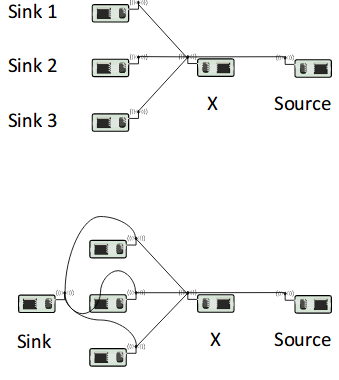
\includegraphics[width=200pt]{two_phase_pull.png}
\end{figure}
For a node X in the figure above here is, at first, only a single option --
remember all neighbors from which an interest message has been received to,
later on once data has been published, forward the actual data to all these
neighbors. In the directed diffusion terminology, this is the setup of
a \textbf{gradient} toward the sender of an interest. Each node stores, for
each type of data received in an interest, in a \textbf{gradient cache}
a separate set of gradients, potentially one for each neighbour. (Gradients
could be bidirectional!) In addition, a gradient is not simply a direction, but
it also contains a value. This value represents, in a sense, the importance or
usefulness of a given link. Initially, these gradient values are the same for
each neighbor; they are modified in the course of the protocol execution. Also,
these gradients are initialized to low values, which are used to explore the
network.

Once the gradients are set up, even with only preliminary values, data can be
propagated. A node that can contribute actual data from local measurements
becomes a source and starts to send data. It uses the highest rate of all its
outgoing gradients to sample and send data. An intermediate node,in the
simplest case, would forward all incoming data messages over all its outgoing
gradients, potentially suppressing some of the data messages to adapt to the
rate of each gradient. This simple scheme, however, results in unnecessary
overhead in the presence of loops in the gradient graph. Hence, the data cache
is introduced: Each node stores, for each known interest, the recently received
data messages. If the same message comes in again -- irrespective of from the
same or different originators -- it is silently discarded.

Even with the data cache, more than one copy of the same data can be delivered
to the sink, constituing some overhead. The gradient values, or more
specifically the rates associated with the gradients, provide a lever to solve
this problem. A neighboring node that contributes new data messages (which
cannot be found in the data cache) should be preferred over neighbors that only
provide stale copies, or rarely provide new data, or appear to have high error
rates, or are otherwise unattractive. This `preference' of a neighbor can
simply be mapped onto the rate of a gradient. A node can reinforce a neighbor
by simply sending a new interest message to that neighbor asking for a higher
rate of data transmission. If this new, required rate is higher that the data
rate that an intermediate node is currently receiving, it in turn can reinforce
its best neighbor with this higher rate. In the end, the reinforcement will
percolate to the source(s) of the data messages.

If the quality of the link between two nodes degrades and events are frequently
corrupted, the receiving node can detect this degradation and can apply
reinforcement rules (which in turn will modify the gradient) to discover a new
best path from source to sink. 
\\
\\
\textit{\circled{9.} Explain why the ``gradient'' concept in directed diffusion
allows to cope with sensor faults.}

Similar to above question, if a receiving node establishes that it is receiving
stale data/no data/outlying data it will just reinforce another neighbour by
asking for a higher data (thus modifying the gradient).
\\
\\
\textit{\circled{10.} Describe Min-T routing and generally link based routing
protocols.}

(N.B. I'm struggling to find description of the protocol, googling "min-t
protocol" gives nonsense. Please provide some resources. Thus, what I'm about
to write will be non-sense as I'm trying to recall the information from the
lecture notes.)

In lossy networks, DVR using hop count only might underestimate costs as the
closest path could be on a bad link and lots of retransmissions may occur.
Thus, Min-T (Minimum Transmission) metric measues expected number of
transmissions along the path. For each link Min-T cost is estimated by
$\frac{1}{Forwad link quality}\times\frac{1}{Backward link quality}$ (Backward
links are important for acks, etc.)

\end{document}
